%%%% Paramétrage du TD %%%%
\def\xxactivite{Révisions \ifprof -- Corrigé \else \fi} % \normalsize \vspace{-.4cm}
\def\xxauteur{\textsl{Xavier Pessoles}}


\def\xxnumchapitre{Révision 1 \vspace{.2cm}}
\def\xxchapitre{\hspace{.12cm} Résolution des problèmes de statique -- Statique 2D}
\def\xxonglet{\textsf{Rév -- Stat}}
\def\xxactivite{TD 01}
\def\xxauteur{\textsl{Xavier Pessoles}}

\def\xxpied{%
Révision statique -- Résolution des problèmes de statique plane\\
Fiche 1 -- \xxactivite%
}

\def\xxcompetences{%
\vspace{-.3cm}
\textsl{%
\textbf{Savoirs et compétences :}\\
%\vspace{-.4cm}
%\begin{itemize}[label=\ding{112},font=\color{ocre}] 
%%\item \textit{Res1.C4 : } Correction
% \item \textit{Res1.C4.SF1 : } Proposer la démarche de réglage d’un correcteur proportionnel
%%proportionnel intégral 
%%et à avance de phase
%\item \textit{Con.C2 : } 	Correction d’un système asservi	
%\item \textit{Con.C2.SF1 : } Choisir un type de correcteur adapté
%\end{itemize}
}}

\def\xxauteur{\textsl{Xavier Pessoles}}

\def\xxtitreexo{Modélisation d'un hayon de coffre électrique}
\def\xxsourceexo{\hspace{.2cm} \footnotesize{Concours Centrale Supelec TSI 2013}}

\def\xxfigures{
\includegraphics[width=.55\textwidth]{fig_00}
}%figues de la page de garde


\iflivret
\input{style/new_pagegarde}
\else
\input{style/new_pagegarde}
\fi
\setlength{\columnseprule}{.1pt}

\pagestyle{fancy}
\thispagestyle{plain}

\vspace{5cm}

\def\columnseprulecolor{\color{ocre}}
\setlength{\columnseprule}{0.4pt} 

\setcounter{exo}{0}

%\ifprof
%%\begin{multicols}{2}
%\else
%\begin{multicols}{2}
%\fi
%%%%%%%%%%%%%%%%%%%%%%%%%%%%%%%%%%%%%%%%%%%%%%%%%%


\section{Les graphes ? Où ça ?}
Réseau de transport, Graphes du web, 
réseaux sociaux, bio-informatique. 

\section{Arbres binaires}

\begin{defi}[Arbres]\cite{ref_01}
Un arbre est un ensemble de \textbf{n\oe{}uds}, organisés de façon hiérarchique, à partir d'un n\oe{}ud distingué appelé racine.
\end{defi}

% définition des styles
\tikzstyle{lien}=[->,>=stealth,rounded corners=5pt,thick]
\tikzset{equipe/.style={draw,thick,fill=#1!25},
equipe/.default={white}}

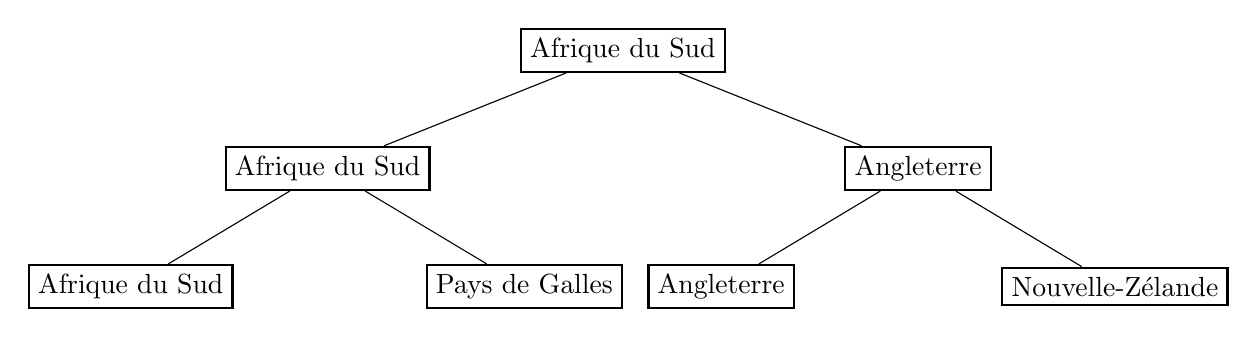
\begin{tikzpicture}[level 1/.style={sibling distance=7.5cm},
level 2/.style={sibling distance=5cm},
level 3/.style={sibling distance=2.5cm}]
\node [equipe] {Afrique du Sud}
	child{ node [equipe]{Afrique du Sud}
		child { node [equipe]{Afrique du Sud}
			%child { node [equipe]{Afrique du Sud}}
			%child { node [equipe]{Japon}}
		}
		child { node [equipe]{Pays de Galles}
			%child { node [equipe]{Pays de Galles}}
			%child { node [equipe]{France}}
			}
		}
	child { node [equipe]{Angleterre}
		child { node [equipe]{Angleterre} 
			%child { node [equipe]{Angleterre}}
			%child { node [equipe]{Australie}}
			}
		child { node [equipe]{Nouvelle-Zélande} 
			%child { node [equipe]{Angleterre}}
			%child { node [equipe]{Australie}}
				}
};
\end{tikzpicture}


\section{}
\begin{defi}[Graphe orienté]

\end{defi}

\begin{defi}[Graphe non orienté]

\end{defi}

\begin{defi}[Sommet -- n\oe{}ud]

\end{defi}

\begin{defi}[Arc]

\end{defi}


\begin{defi}[Arête]

\end{defi}


\begin{defi}[Boucle]

\end{defi}


\begin{defi}[Degré entrant et sortant]

\end{defi}



\begin{defi}[Chemin d'un sommet à un autre]

\end{defi}


\begin{defi}[Cycle]

\end{defi}


\begin{defi}[Connexité dans les graphes non orientés]

\end{defi}







\ref{01}{Types de données algorithmes, Christine Froidevaux, Marie-Christine Gaudel, Michèle Soria. Mc Graw -- Hill.}